\documentclass{../exhibit}

\title{Look at me Gems}

%% Font
\usepackage{imfellEnglish}
\usepackage[T1]{fontenc}
\raggedright

\usepackage{background}

\backgroundsetup{
scale=1,
color=black,
opacity=0.4,
angle=0,
contents={%
  \includegraphics[height=\paperheight]{mapBackground.jpg}%%https://upload.wikimedia.org/wikipedia/commons/8/81/Nautical_chart_of_the_West_Indies_1797.jpg
  }%
}




%% For the context
%% https://tex.stackexchange.com/questions/86150/torn-page-effect/86151#86151
\usepackage{tikz}
\usetikzlibrary{decorations.pathmorphing}
\definecolor{paper}{RGB}{239,227,157}





\renewcommand{\maketitle}{ %
  \begin{center}
    \scalebox{8}{\thetitle}
  \end{center}
  
\begin{tabular*}{\textwidth}{c @{\extracolsep{\fill}} c}  
\resizebox{4in}{!}{\begin{minipage}[b]{3in}\huge\directions\end{minipage}} &
  \resizebox{4in}{!}{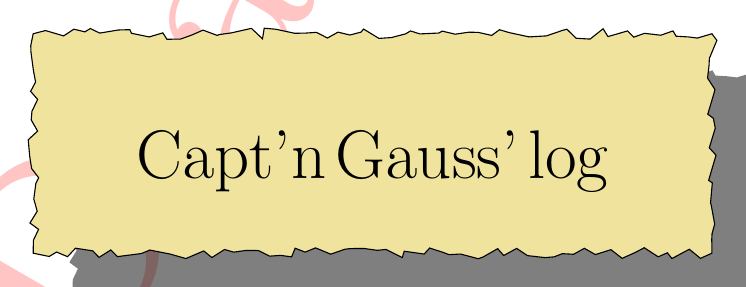
\begin{tikzpicture}[pencildraw/.style={ %
    decorate,
    decoration={random steps,segment length=4pt,amplitude=2pt}
    } %
]
\node[
preaction={fill=black,opacity=.5,transform canvas={xshift=.5cm,yshift=-.5cm}},
pencildraw,draw,fill=paper,text width=3in,inner sep=.5cm] 
{\begin{center}\Huge Capt'n Gauss' log \end{center}\vspace{.7cm} {\huge\context}};
\end{tikzpicture}}

\end{tabular*}

\vfill

\includegraphics[width=3in]{logoPirate.png}\hfill \includegraphics[width=2in]{bammLogo.png}


}


\begin{document}


\begin{context} Arr, Euler be known as the ``Mathematical pirate''
among his peers, fer his ability to plunder new mathematical treasure
and discover hidden gems.  Euler also discovered ``Euler
characteristic'' and in this task, you'll be discovering this as well.

In this here task, ye need to be countin' the number o' corners,
number o' faces, and number o' edges on various shapes. Ye best be
jotting down that information on yer worksheet, lest ye forget! Ye'll
be needin' to pay close attention and use yer pirate skills o'
observation to spot all the details on them shapes. Remember, a good
pirate always keeps track o' their loot!
\end{context}


\begin{directions}
  For each polyhedron,
  \begin{itemize}
  \item count the number of corners (``vertices''),
  \item count the number of flat faces,
  \item and count the number of edges.
  \end{itemize}
  Record this on your worksheet.  \textbf{What patterns do you see?}
\end{directions}



\begin{example}

For example, if you take a cube, it has 8 corners (vertices), 12 edges, and 6 faces.
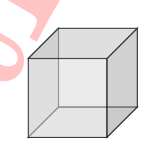
\begin{tikzpicture}
\draw[fill=gray!40,opacity=0.5] (0,0,0) -- (1,0,0) -- (1,0,1) -- (0,0,1) -- cycle;
\draw[fill=gray!20,opacity=0.5]  (0,0,0) -- (0,1,0) -- (1,1,0) -- (1,0,0) -- cycle;
\draw[fill=gray!60,opacity=0.5]  (0,0,0) -- (0,0,1) -- (0,1,1) -- (0,1,0) -- cycle;
\draw[fill=gray!20,opacity=0.5]  (0,0,1) -- (0,1,1) -- (1,1,1) -- (1,0,1) -- cycle;
\draw[fill=gray!60,opacity=0.5]  (1,0,0) -- (1,0,1) -- (1,1,1) -- (1,1,0) -- cycle;
\draw[fill=gray!40,opacity=0.5]  (0,1,0) -- (1,1,0) -- (1,1,1) -- (0,1,1) -- cycle;
\end{tikzpicture}
\end{example}



\begin{mathConnections}
  https://bartsnapp.github.io/Math-Outreach-Exhibits/eulerCharacteristic/
\end{mathConnections}
\end{document}
